%\documentclass[preprint]{sigproc}
\documentclass{acm_proc_article-sp}

% The following \documentclass options may be useful:
%
% 10pt          To set in 10-point type instead of 9-point.
% 11pt          To set in 11-point type instead of 9-point.
% authoryear    To obtain author/year citation style instead of numeric.

\setlength{\textfloatsep}{5pt}

\usepackage{flushend}
\usepackage{graphicx}
\usepackage{verbatim}
\usepackage{url}
\usepackage{alltt}
\renewcommand{\ttdefault}{txtt}

\usepackage{amsmath}
\usepackage{dsfont}
\usepackage{mathtools}
\everymath{\displaystyle}
\usepackage{xspace}

\newcommand{\CEU}{\textsc{C\'{e}u}\xspace}
\newcommand{\code}[1] {{\small{\texttt{#1}}}}
\newcommand{\DOFIN}{\code{do-finally}\xspace}
\newcommand{\FIN}{\code{finally}\xspace}

\newcommand{\ST}{\1\xrightarrow[~n~]{}\1}
\newcommand{\BT}{\xRightarrow[(i,E)]{}}
\newcommand{\LL}{\langle}
\newcommand{\RR}{\rangle}
\newcommand{\DS}{\displaystyle}
\newcommand{\rr}[1] {{\textbf{\scriptsize{#1}}}}


\newcommand{\1}{\;}
\newcommand{\2}{\;\;}
\newcommand{\3}{\;\;\;}
\newcommand{\5}{\;\;\;\;\;}
\newcommand{\ten}{\5\5}
\newcommand{\twenty}{\ten\ten}

\newenvironment{itemize*}%
  {\begin{itemize}%
    \setlength{\itemsep}{0pt}%
    \setlength{\parskip}{0pt}}%
  {\end{itemize}}

\usepackage{enumitem}
\setlist{nolistsep}

\usepackage{color}
\definecolor{light}{gray}{0.87}
\definecolor{dark}{gray}{0.30}
%\definecolor{light}{rgb}{.90,.90,.90}
\definecolor{darkgreen}{rgb}{0,.50,0}
\definecolor{darkblue}{rgb}{0,0,.50}
\definecolor{darkred}{rgb}{.50,0,0}
\definecolor{darkpur}{rgb}{.50,0,.50}

\usepackage{listings}
%\usepackage{textcomp}
\lstset{
%columns=fullflexible,
%basicstyle=\ttfamily,
escapeinside={||},
mathescape=true,
    language=C, % choose the language of the code
    basicstyle=\fontfamily{pcr}\selectfont\scriptsize\color{black},
    keywordstyle=\color{black}\bfseries, % style for keywords
    numbers=none, % where to put the line-numbers
    numberstyle=\tiny, % the size of the fonts that are used for the line-numbers
    backgroundcolor=\color{light},
    showspaces=false, % show spaces adding particular underscores
    showstringspaces=false, % underline spaces within strings
    showtabs=false, % show tabs within strings adding particular underscores
    %frame=single, % adds a frame around the code
    tabsize=2, % sets default tabsize to 2 spaces
    %rulesepcolor=\color{gray}
    captionpos=t, % sets the caption-position to bottom
    breaklines=false, % sets automatic line breaking
    %breakatwhitespace=false,
    numbersep=2em,
    emph={par,or,hor,do,end,loop,await,emit,input,event,call,with,command,%
          var,and,then,else,C,return,pure,deterministic,nohold,finalize,%
          class, every, FOREVER, this,
          each, abort, when, signal, PROC, CHAN, SIGNAL, PAR},
    emphstyle={\bfseries},
    commentstyle=\color{dark}\scriptsize,
    %xleftmargin=20pt,
    %xrightmargin=20pt,
    framesep=20pt,
    %upquote=true,
    %aboveskip={1.5\baselineskip},
}

\begin{document}

\title {
    %Imperative and Synchronous Abstractions for Reactive Applications
    Abstract and Structured Reactive Programming
}
%\subtitle{Accepted paper in REM'13 (preprint version)}

\numberofauthors{1}
\author{
    \alignauthor
    Francisco Sant'Anna \hspace{1cm} Noemi Rodriguez \hspace{1cm} Roberto Ierusalimschy   \\
    \affaddr{Departamento de Inform\'atica --- PUC-Rio, Brasil} \\
    \email{\{fsantanna,noemi,roberto\}@inf.puc-rio.br}
}

\maketitle

\begin{abstract}
.......... ........... ........... ........... ........... ...........
.......... ........... ........... ........... ........... ...........
.......... ........... ........... ........... ........... ...........
.......... ........... ........... ........... ........... ...........
.......... ........... ........... ........... ........... ...........
.......... ........... ........... ........... ........... ...........
.......... ........... ........... ........... ........... ...........
.......... ........... ........... ........... ........... ...........
.......... ........... ........... ........... ........... ...........
.......... ........... ........... ........... ........... ...........
\end{abstract}

%\category{CR-number}{subcategory}{third-level}
%\category{D.3.1}{Programming Languages}{Formal Definitions and Theory}
%\category{D.3}{Programming Languages}{General}
\category{D.3.3}{Programming Languages}{Language Constructs and Features}

\terms{Design, Languages}

\keywords{Concurrency, Determinism, Esterel, Imperative, Structured 
Programming, Synchronous, Reactivity}

\section{Introduction}
\label{sec.intro}

Reactive applications interact continuously and in real time with external 
stimuli from the environment.
They represent a wide range of software areas and platforms: from games in 
powerful desktops, ``apps'' in capable smart phones, to the emerging internet 
of things in constrained embedded systems.

Research on special-purpose reactive languages dates back to the early 80's 
with the co-development of two complementary 
styles~\cite{rp.twelve,rp.hypothesis}:
%
The imperative style of Esterel~\cite{esterel.ieee91} organizes programs with 
structured control flow primitives, such as sequences, repetitions, and 
parallelism.
%
The dataflow style of Lustre~\cite{lustre.ieee91} represents programs as graphs 
of values, in which a change to a node updates its dependencies automatically.

In recent years, Functional Reactive Programming~\cite{frp.principles} 
modernized the dataflow style and became mainstream, deriving a number of 
languages and libraries, such as Flapjax~\cite{frp.flapjax}, Rx (from 
Microsoft), React (from Facebook), and Elm~\cite{frp.elm}.
%
In contrast, the imperative style did not follow this trend and is now confined 
to the domain of real-time embedded control systems.
% such as flight control on avionics and anti-collision equipment on automobiles.

As a matter of fact, imperative reactivity is now often associated to the 
\emph{observer pattern}, typical in object oriented systems, because it heavily 
relies on side effects over objects~\cite{rp.deprecating,rp.rescala}.
%
However, short-lived callbacks (i.e., the observers) eliminate any vestige of 
structured programming, such as support for loops and automatic 
variables~\cite{sync_async.cooperative}, which are elementary capabilities of 
imperative languages.
%
In this sense, the observer pattern actually disrupts imperative reactivity, 
becoming ``our generation's \code{goto}''~\cite{dij.goto,rp.goto,elm.goto}.

In this work, we revive the synchronous imperative programming style of 
Esterel, which we now refer as \emph{Structured Reactive Programming (SRP)}.
%
SRP extends classical structured programming (SP)~\cite{dij.notes} to support 
continuous interaction with the environment through hierarchical flow 
constructs: \emph{concatenation}, \emph{selection}, \emph{repetition}, and also 
\emph{parallelism}.
%
Concretely, we consider that SRP must provide at least two fundamental 
extensions to SP:
%
\begin{itemize}
\item An \code{await <evt>} statement that suspends a line of execution until 
the referred event occurs, keeping the whole data and control context alive.
\item Parallel constructs that compose multiple lines of execution and make 
them concurrent.
\end{itemize}
%
The \code{await} statement captures the imperative and reactive nature of SRP, 
recovering from the inversion of control inherent to the observer pattern, and 
thus restoring sequential execution and support for automatic variables.
Parallel compositions allow for multiple \code{await} statements to coexist, 
which is necessary to handle concurrent events common in reactive applications.

Our main contribution is a new mechanism for SRP, named as \emph{organisms}, 
that abstracts parallel and \code{await} statements and offer an object-like 
interface that other parts of the program can manipulate.
%
In brief, organisms are to SRP like procedures are to SP, i.e., one can 
abstract a portion of code with a name and ``call'' that name from multiple 
places.
%
There are, however, some semantic challenges that apply to organisms:
%
\begin{itemize}
\item An organism is part of a concurrent program that can manipulate it and 
affect its data and execution state.
\item An organism is itself alive and concurrent, essentially forking the 
calling line of execution to also accommodate it.
\item An organism can be static or dynamic. Dynamic instances require a memory 
management model.
\end{itemize}

We support organisms in the programming language \CEU~\cite{ceu.sensys13}.
%
\CEU is based on Esterel and relies on a similar synchronous and deterministic 
execution model that simplifies the reasoning about concurrency aspects.
%
We propose a memory model for organisms that eliminates known issues in dynamic 
allocation: \emph{memory leaks}, \emph{dangling pointers}, and the need for 
\emph{garbage collection}.
%
The model is similar to stack-living local variables of procedures, providing 
lexical scope and automatic bookkeeping of organisms.
We also restrict explicit references to organisms to avoid indirect 
manipulation.

\begin{comment}

TODO

= CONCLUSION
Overall, organisms reconcile data and control state in a single concept.
\CEU provides a contemporary outlook of SRP that aims to expand its application 
domain.
these languages shows that imperative can be safe with a reasonable concurrency 
model and static analysis

= CEU
sintaxe (separar section 1 / 2)

\end{comment}

The rest of the paper is organized as follows:
Section~\ref{sec.synchronous} reviews the synchronous and asynchronous 
execution model, justifying the former as a better choice for SRP.
Section~\ref{sec.ceu} presents SRP through \CEU, with its basic control 
mechanisms and the organisms abstraction.
Section~\ref{sec.demo} demonstrates a complete video game for Android 
implemented in \CEU.
Section~\ref{sec.related} discusses related work.
Section~\ref{sec.conclusion} concludes the paper and makes final remarks.

\section{The Synchronous Concurrency Model}
\label{sec.synchronous}

``Reactive systems'' are not a new class of software and have been first 
described by Harel as being ``repeatedly prompted by the outside world and 
their role is to continuously respond to external 
inputs''~\cite{statecharts.reactive}.
In comparison to traditional ``transformational systems'', he recognises 
reactive systems as ``particularly problematic when it comes to finding 
satisfactory methods for behavioral description''.
%
Berry goes further and makes a subtle distinction between ``interactive'' and 
``reactive'' systems~\cite{rp.synchronous}:
%
\begin{itemize}
\item Interactive programs interact at their own speed with users or with other 
programs; from a user point of view a time-sharing system is interactive.
\item Reactive programs also maintain a continuous interaction with their 
environment, but at a speed which is determined by the environment, not by the 
program itself.
\end{itemize}

%He states that ``interactive programs work at their own pace and mostly deal 
%with communications, while reactive programs only work in response to external 
%demands and mostly deal with accurate interrupt handling.''

This distinction is fundamental because the different control perspectives 
(i.e., \emph{at the speed of the program} vs \emph{at the speed of the 
environment}) implies the use of different underlying concurrency models.
%
Overall, \emph{synchronous languages} deal with reactive systems better, while 
\emph{asynchronous languages}, with interactive systems~\cite{esterel.crp}.
%
Both mentioned authors propose synchronous languages for designing reactive 
systems (Statecharts~\cite{statecharts.visual} and 
Esterel~\cite{esterel.ieee91}).

%%%%%%%%%%%%%%%%%%%%%%%%%%%%%%%%%%%%%%%%%%%%%%%%%%%%%%%%%%%%%%%%%%%%%%%%%%%%%%%

The synchronous execution model is based on the hypothesis that internal 
computations (\emph{reactions}, in this context) run infinitely faster than the 
rate of events that trigger them.
In other words, the input and corresponded output are simultaneous, because 
reactions takes no time.

\begin{figure}
\centering
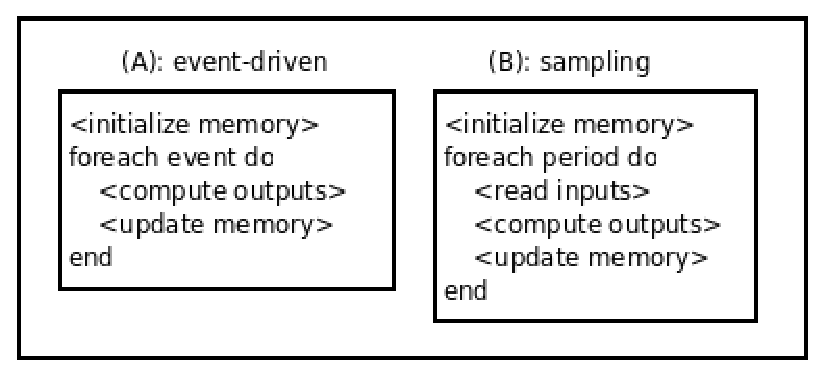
\includegraphics[width=3.0in]{sync_impl.eps}
\caption{Schedulers for synchronous systems}
\label{fig.impl}
\end{figure}
% Esterel, HW, \CEU, observers

Figure \ref{fig.impl} shows two common implementation schemes for synchronous 
schedulers~\cite{rp.twelve}.
%
In the event-driven scheme, a loop iteration computes outputs for each event 
occurrence.
%
In the sampling scheme, a loop iteration computes the inputs and outputs on 
every clock tick.
%
In both cases, each loop iteration represents a logical instant in which the 
system as a whole reacts synchronously before going to the next instant.
%
During a reaction, the environment is invariant and does not affect the running 
iteration%
\footnote{
An actual implementation enqueues incoming input events to process them in the 
next iterations.
}.
%
Both schemes are compliant with the synchronous hypothesis, in which input and 
resulting output happen at the same time, considering this notion of time as a 
sequence of discrete events or clock ticks.

The asynchronous execution model is more general and does not make assumptions 
about implicit synchronization.
Each activity in the system%
\footnote{We use the term activity to generically refer to a language's unit of 
execution (e.g., \emph{thread}, \emph{actor}, \emph{process}, etc.).}
is independent from one another and executes at its own pace.
%
For instance, an activity can perform time-consuming operations (e.g., 
compression, cryptography) without affecting the overall progress of the 
system.
%
This separation also makes many-core parallelism straightforward.
%
However, in order to coordinate at specific points, the activities require 
explicit synchronization primitives (e.g., mutual exclusion or message 
passing).
% ADA, thread-based concurrency, CSP

%%%%%%%%%%%%%%%%%%%%%%%%%%%%%%%%%%%%%%%%%%%%%%%%%%%%%%%%%%%%%%%%%%%%%%%%%%%%%%%

In this work, we emphasize two desired features in concurrent systems that the 
synchronous model makes possible: \emph{deterministic execution} and 
\emph{orthogonal abortion}.
%
In the context of reactive applications, we interpret determinism as 
\emph{reproducible execution given the same sequence of stimuli}, i.e., the 
outcome depends exclusively of an external input timeline, in contrast with 
internal scheduling and communication timings.
%
Orthogonal abortion is the ability to abort an activity (from outside it) 
without affecting the overall consistency of the system (e.g., properly 
releasing global resources).

\begin{comment}
%
Having the language to deal automatically with these features strengthen 
structured programming, because we can compose activities together.
%
For instance, although adding a new activity implies extra computational 
overhead, it does not affect the behavior of the other activities, which still 
depend only on the input timeline.
%
Furthermore, if we want to abort an existing activity given a new requirement, 
we can do it externally, without changing

 determinism and abortion with these issues is interesting allows to
compose activities while keeping them decoupled, because they need not to be 
NOtweaked to accommodate these requirements.


decoupling =>
structured programming

deterministic,
    reproducible
abortion
    structured programming
    no coupling
    just like

The way each side is implemented does not affect the behavior,
only the way you compose them (which is external to each implementation)

%
DET and ABRT
both yield to better reasoning
behave the same with or without concurrency
\end{comment}

%%%%%%%%%%%%%%%%%%%%%%%%%%%%%%%%%%%%%%%%%%%%%%%%%%%%%%%%%%%%%%%%%%%%%%%%%%%%%%%

Figure~\ref{lst.leds} shows three implementations for an application that 
blinks two LEDs in parallel with different frequencies.
We use two asynchronous languages (a CSP-based~\cite{arduino.occam} and a 
thread-based~\cite{arduino.chibios} language), and also the synchronous 
language \CEU.
%
The intent and syntactic structure of the implementations are similar:
composing the two blinking activities in parallel.
%
The LEDs should blink together every 3 seconds (the least common denominator 
between 600ms and 1s).
%
As we expected, the LEDs in the two asynchronous implementations loose 
synchronism after some time of execution, while the implementation in \CEU 
remains synchronized forever.
%
The example highlights how the inherent non-determinism in the asynchronous 
model makes hard to (blindly) compose activities supposedly synchronized: 
unpredictable scheduling as wall as latency in message-passing eventually cause 
observable asynchronism.
%
In \CEU, the \code{await} is the only primitive that takes time, but which the 
programmer uses explicitly to conform with the problem specification.
The internal timings for communication and computation, which the programmer 
cannot control, are neglected in accordance to the synchronous hypothesis.
The language runtime compensates them in the subsequent reaction in order to 
conform with the model and remain synchronized~\cite{ceu.sensys13}.
%
Arguably, reasoning over \code{await} statements is simpler than also having to 
consider all statements of the language.

\begin{figure}[t]
\begin{minipage}[t]{0.34\linewidth}
\begin{lstlisting}
// OCCAM-PI
PROC main ()
 CHAN SIGNAL s1,s2:
 PAR
  PAR
   tick(600, s1!)
   toggle(11, s1?)
  PAR
   tick(1000, s2!)
   toggle(12, s2?)
:

\end{lstlisting}
\end{minipage}
%
\begin{minipage}[t]{0.33\linewidth}
\begin{lstlisting}
// ChibiOS
void thread1 () {
  while (1) {
    sleep(600);
    toggle(11);
  }
}
void thread2 () {
  while (1) {
    sleep(1000);
    toggle(12);
  }
}
void setup () {
  create(thread1);
  create(thread2);
}

\end{lstlisting}
\end{minipage}
%
\begin{minipage}[t]{0.31\linewidth}
\begin{lstlisting}
// Ceu
par do
  loop do
    await 600ms;
    _toggle(11);
  end
with
  loop do
    await 1s;
    _toggle(12);
  end
end
\end{lstlisting}
\end{minipage}
%
\rule{8.5cm}{0.37pt}
\caption{ Two blinking LEDs in OCCAM-PI, ChibiOS and \CEU.\newline
{\small %\textmd{
The lines of execution in parallel blink two LEDs (connected to ports 11 and 
12) with different frequencies.
Every 3 seconds the LEDs should light on together.
}%}
\label{lst.leds}
}
\end{figure}

%%%%%%%%%%%%%%%%%%%%%%%%%%%%%%%%%%%%%%%%%%%%%%%%%%%%%%%%%%%%%%%%%%%%%%%%%%%%%%%

\begin{figure}[t]
\begin{lstlisting}
par/or do
    // activity A
    <local-variables>
    <body>
with
    // activity B
    <local-variables>
    <body>
end
<local-variables>
\end{lstlisting}
\caption{ A \code{par/or} composes two concurrent activities and rejoins when 
one terminates, aborting the other.\newline
{\small %\textmd{
%TODO
}%}
\label{lst.abortion}
}
\end{figure}

Consider now the problem of aborting an \emph{activity A} as soon as an
\emph{activity B} terminates, and vice versa.
%
Figure~\ref{lst.abortion} shows the hypothetical construct \code{par/or} that 
composes concurrent activities and rejoins when either of them terminates, 
properly aborting the other.
%
The \code{par/or} is regarded as an orthogonal abortion construct, because the 
composed activities do not know when and how they are aborted (i.e., abortion 
is external to them).
%
In the example, each activity has a set of local variables and an execution 
body that lasts for an arbitrary time.
After the \code{par/or} rejoins, a new set of local variables goes alive, 
supposedly reusing the space from the activities' locals going out of scope.

Orthogonal abortion in asynchronous languages is 
challenging~\cite{esterel.preemption}.
%
For instance, when an activity terminates, the other activity to be aborted 
might be on a inconsistent state (e.g., suspended but holding a lock, or 
actually executing in another core).
%
In order to properly abort an activity, the language runtime has two possible 
semantics for the \code{par/or}:
either wait to rejoin (delayed termination);
or rejoin immediately and wait in the background (immediate termination).
Both options have problems:
\begin{itemize}
\item \textbf{delayed}:
    The program becomes unresponsive in the meantime.
\item \textbf{immediate}:
    The programmer may assume that both activities have terminated.
    Also, local variables need to coexist in memory for some time, moving the 
    language allocation strategy to the heap (which is discouraged in the 
context of embedded systems).
\end{itemize}

As matter of fact, asynchronous languages do not provide effective abortion:
CSP only supports a composition operator that ``terminates when all of the 
combined processes terminate''~\cite{async.csp};
Java's \code{Thread.stop} primitive has been officially 
deprecated~\cite{sync_async.threadsstop};
and pthread's \code{pthread\_cancel} does not guarantee immediate 
cancellation~\cite{sync_async.pthreadsstop}.
%
Instead, asynchronous activities typically agree a on common protocol to abort 
each other (e.g., through shared state variables or message passing).

Synchronous languages, however, provide accurate control over the life cycle of 
concurrent activities, because in between every reaction, the whole system is 
idle and consistent~\cite{esterel.preemption}.
%
\CEU provides the presented \code{par/or} composition, which is equivalent to 
Esterel's \code{trap} orthogonal abortion construct.
%
We show in Section~\ref{sec.ceu} how abortion integrates safely with activities 
that use stateful resources from the environment, such as file handling and 
network transmissions.

%%%%%%%%%%%%%%%%%%%%%%%%%%%%%%%%%%%%%%%%%%%%%%%%%%%%%%%%%%%%%%%%%%%%%%%%%%%%%%%

Even tough the deterministic and abortion examples can be properly implemented 
in asynchronous languages, they require to tweak the activities with mutual
synchronization primitives.
%
This increases the coupling degree among activities with concerns that are not 
directly related to the problem specification.

The two models suggest a tradeoff between unrestricted execution with real 
parallelism versus structural composability with deterministic behavior.
%
For reactive applications with continuous and real-time concurrency, we believe 
that the synchronous execution model is more appropriate.

\begin{comment}

On the other hand, the synchronous hypothesis does not hold for reactions that 
have latency (e.g., network communication or algorithm-intensive computations),
however, does not apply when the computation involves latency:
problem communication takes time
either communication or time consuming operations
because now, at the speed of the program

parallelism
latency

For reactive systems zzz
For highly synchronous systems, the sole synchronization overhead, which is 
non-existent in XXX, may neutralize any gains with parallelism.
% or even worsen parallelism

Illustrate with two examples:
that explore the advantages of synchronous:
reasoning in concurrency
seamless composition

communitacions is directed and takes time (because the receiver may not be 
waiting)

The synchronous model
input => output
broadcast possible
global consensus possible
determinism
simpler model

In synchronous systems, communication is instantaneous.
The zero-delay property of the synchronous hypothesis guarantees that no time 
elapses between event announcement and receiving.
Also, as communication is via broadcast, all systems parts share the same 
information all the time.
These two characteristics make global data consensus another property of 
synchronous systems.

conclusion:
no blind/free/orthogonal composition
no deterministic/reproducible execution
parallelism / no-forced synch
time-consuming / independent

A recent Reactive Manifesto

synchronous reactive
vs
asynchronous reactive

\end{comment}

\section{Structured Reactive Programming with C\'eu}
\label{sec.ceu}

- intro
- example
- model

\subsection{Compositions}

- besides standard strucutred (loops, conditionals, sequences)
- add compositions
- await, sequence, vars
- parallel, patterns, ortoghonal

\subsubsection{Finalization}

- finalize for C integration and keep orthogonality
- no await inside it

\subsection{Organisms}

So far, no abstractions

Organisms are an abstraction mechanism that reconciles data and control state 
into the single concept.
Organisms provide an object-like interface (data state) as well as multiple 
lines of execution (control state).
The syntax xxx

A class of organisms is composed of an interface and a single execution body.  
The interface exposes public variables, methods, and internal events, like in 
object oriented programming.
The body can contain any valid code in Céu (including parallel compositions) 
and starts on organism instantiation, executing in parallel with the program.  
Organism instantiation can be either static or dynamic.

The example of Figure~\ref{lst.orgs} introduces static organisms through three 
code chunks:
%
\begin{itemize}
\item The leftmost code is a modified version of the two blinking LEDs of 
Figure~\ref{lst.leds} that terminates after 1 minute.
%
\item The code in the middle abstracts the blinking LEDs in an organism class 
and uses two instances to reproduce the same behavior.
%
\item The rightmost code is the equivalent expansion that removes organisms, 
which should resemble the original leftmost code.
\end{itemize}
%
The Blink class (lines 1-11) exposes the led and freq fields, which correspond 
to the LED port and blinking frequency to be configured for each instance. The 
application creates two instances, specifying the fields in the constructors 
(lines 13-16 and 18-21). A constructor starts the instance body to execute in 
parallel with the application. When reaching the await 1min (line 23), each 
instance already has its body switching between \_on() and \_off() every freq 
milliseconds (lines 5-10).

The code in the left is semantically equivalent to the one in the right, which 
expands the organisms bodies (lines 13-18 and 22-27) in a par/or with the rest 
of the application (await 1min, in line 30). Note the await FOREVER statements 
(lines 19 and 28) that avoid the organisms bodies to terminate the par/or. The 
\_Blink type corresponds to a simple datatype without execution body (i.e., 
conventional structs or records or objects).

\begin{figure*}[t]
\begin{minipage}[t]{0.28\linewidth}
\begin{lstlisting}
par/or do
    every 600ms do
        _toggle(11);
    end
with
    every 1s do
        _toggle(12);
    end
with
    await 1min;
end


















  /* Original blink */
\end{lstlisting}
\end{minipage}
%
\begin{minipage}[t]{0.30\linewidth}
\begin{lstlisting}[numbers=left,xleftmargin=1.0em]
class Blink with
    var int port;
    var int dt;
do
    every (dt)ms do
        _toggle(port);
    end
end

do
    var Blink b1 with
        this.port = 11;
        this.dt   = 600;
    end;

    var Blink b2 with
        this.port = 12;
        this.dt   = 1000;
    end;

    await 1min;
end







  /* Blink organism */
\end{lstlisting}
\end{minipage}
%
\begin{minipage}[t]{0.32\linewidth}
\begin{lstlisting}[numbers=left,xleftmargin=1.0em]
struct _Blink with
    var int port;
    var int dt;
end;

do
    var _Blink b1, b2;

    par/or do
        // body of b1
        b1.port = 0;
        b1.dt   = 2;
        every (b1.dt)ms do
            _toggle(b1.port);
        end
        await FOREVER;
    with
        // body of b2
        b2.port = 1;
        b2.dt   = 4;
        every (b2.dt)ms do
            _toggle(b2.port);
        end
        await FOREVER;
    with
        await 1min;
    end
end

  /* Organism expansion */
\end{lstlisting}
\end{minipage}
%
\rule{17.5cm}{0.37pt}
\caption{ Two blink LEDs using organisms.\newline
{\small %\textmd{
In a realistic example, the textual overhead of a class should payoff.
}%}
\label{lst.orgs}
}
\end{figure*}

\subsubsection{Dynamic Organisms}

- organisms, static, dynamic. do T;

\section{Related work}

- asynchronous langs
- Esterel + descendants
- CRP
- simula
- FRP

interactive  vs reactive
asynchronous vs synchronous
dataflow vs control
dynamic vs static

imperative
    - sequential (eliminates state machines)
    - better resource control
    - less abstract

dataflow

exemplo data melhor vs control melhor

The synchronous concurrency model...

We show composibility, sequential, imperative
safety
Then, we extend synchronous reactive programming with dynamic

control vs data reactivity

\begin{comment}
===============================================================================

In computing, reactive programming is a programming paradigm oriented around data flows and the propagation of change. This means that it should be possible to express static or dynamic data flows with ease in the programming languages used, and that the underlying execution model will automatically propagate changes through the data flow.

For example, in an imperative programming setting, a := b + c would mean that a is being assigned the result of b + c in the instant the expression is evaluated. Later, the values of b and c can be changed with no effect on the value of a.

In reactive programming, the value of a would be automatically updated based on 
the new values.

===============================================================================

There seems to be a lot of confusion about Reactive Programming. What is it? Who created it?

The earliest reference I could find was written by Gérard Berry (one of the creators of the Esterel dataflow language) in his 1989 paper, “Real time programming: Special purpose or general purpose languages.” I emailed him to see if he knew of an earlier use. Mr. Berry pointed me to the 1985 paper, “On the development of reactive systems” by David Harel and Amir Pnueli. After contacting Professor Harel, he confirmed that they where the originators of the term.

So it would seem that Reactive Programming is at least 30 years old.

Harel and Pnueli’s paper discussed designing reactive systems in general, software or hardware. Their definition was…

    “Reactive systems… are repeatedly prompted by the outside world and their role is to continuously respond to external inputs.”

    D. Harel and A. Pnuli, “On the Development of Reactive Systems” (1985)

Mr. Berry’s paper focused on the software aspects of Reactive Programming…

    “It is convenient to distinguish roughly between three kinds of computer programs. Transformational programs compute results from a given set of inputs; typical examples are compilers or numerical computation programs. Interactive programs interact at their own speed with users or with other programs; from a user point of view a time-sharing system is interactive. Reactive programs also maintain a continuous interaction with their environment, but at a speed which is determined by the environment, not by the program itself. Interactive programs work at their own pace and mostly deal with communications, while reactive programs only work in response to external demands and mostly deal with accurate interrupt handling.

    Real-time programs are usually reactive. However, there are reactive program that are not usually considered as being real-time, such as protocols, system drivers or man-machine interface handlers. All reactive programs require a common programming style.

    Complex applications usually require establishing cooperation between the three kinds of programs. For example, a programmer uses a man-machine interface involving menus, scroll bars and other reactive devices. The reactive interface permits him to tell the interactive operating systems to start transformational computations such as program compilations.”

    Berry, Gérard. “Real time programming: Special purpose or general purpose languages.” (1989)

From the preceding quotes we can say that reactive programs…

    Activate in response to external demands
    Mostly deal with handling parallelism
    Operate at the rate of incoming data
    Often work in cooperation with transformational and interactive aspects

The definition of dataflow is a little more vague. Any system where the data moves between code units and triggers execution of the code could be called dataflow, that includes reactive systems. Thus, I consider Reactive Programming to be a subset of dataflow but a rather large subset. In casual use, Reactive Programming it is often a synonym for dataflow.

In more recent years Reactive Programming has become associated with two elements. Microsoft’s Reactive Extensions and Typesafe’s Reactive Manifesto.

Some people believe that Erik Meijer (formerly of Microsoft) and Jonas Bonér (of Typesafe) are trying to claim an old idea and call it their own. I am quite sure both of them are very aware of all of the previous work that has gone into Reactive Programming and dataflow. Mr. Bonér wrote about his observations on the resurgence of old techniques to solve new problems…

    “…Over the last few years we have seen quite a few different techniques and tools emerge in the industry as a way to address these new requirements. Some of them are old and proven, but to a large extent forgotten techniques, while others are novel and creative.”

    Why Do We Need a Reactive Manifesto

Reactive Programming and dataflow are old ideals that are being rediscovered because they help us solve problems we currently face.
\end{comment}

Adding dynamic state and references to SRP is a significant contribution.  
However the presentation assumes the audience already appreciates the 
advantages of SRP over standard imperative semantics. Most observers will not 
notice the difference at all and think this is just a weird syntactic sugar for 
standard multithreaded programming. SRP needs to be better explained and 
justified, perhaps by showing how it simplifies the examples.

\CEU is a Esterel-based reactive language that targets constrained embedded 
platforms.
%
Relying on a deterministic semantics, it provides safe shared-memory 
concurrency among lines of execution.
%
\CEU introduces a stack-based execution policy for internal events which 
enables advanced control mechanisms considering the context of embedded 
systems, such as exception handling and a limited form of coroutines.
%
The conjunction of shared-memory concurrency with internal events allows 
programs to express dependency among variables reliably, reconciling the 
control and dataflow reactive styles in a single language.
%As far as we know, \CEU is the first language to reconcile the control and 
%dataflow reactive styles.
%
%We present a formal description of \CEU and show how its synchronous and 
%static nature enables a compile-time analysis to ensure that reactions to the 
%environment are deterministic and execute with bounded memory and CPU time.

\bibliographystyle{abbrv}
\bibliography{other,my}

\end{document}
